\documentclass[11pt]{article}
\usepackage[review]{acl}
\usepackage{times,latexsym}
\usepackage[T1]{fontenc}
\usepackage[utf8]{inputenc}
\usepackage{microtype,inconsolata}
\usepackage{amsmath,amssymb}
\usepackage{graphicx,booktabs,multirow,tabularx,array}
\usepackage{placeins,xurl}
\newcommand{\pending}{\textemdash}
\title{Evidence Grounding and Strategy Evolution for Agent Task Generation from Longitudinal EHRs}
\author{}
\hypersetup{pdftitle={Evidence Grounding and Strategy Evolution for Agent Task Generation from Longitudinal EHRs},pdfauthor={}}
\begin{document}
\maketitle
\begin{abstract}
Generating high-quality tasks for medical agents from longitudinal EHRs is challenging because patient records differ in the clinical relationships they support, while available tools restrict how evidence can be retrieved. Here, we propose MedEvolve, a framework that improves medical task generation at two complementary levels, task grounding and strategy evolution. At the task-construction level, dual exploration distills recurring clinical-temporal patterns and tool-access constraints into reusable guidance. At the strategy level, feedback-driven evolution then converts verification and independent-solving outcomes into cross-patient construction rules and task-direction preferences, rather than only repairing individual questions.
MedEvolve achieves higher verified higher-order task yield than the baselines on both benchmarks. Adding its synthetic tasks improves official-test success rates by 6 and 2 percentage points for ACE and Reflexion, respectively.
\end{abstract}

\section{Introduction}

\begin{figure*}[!t]
\centering
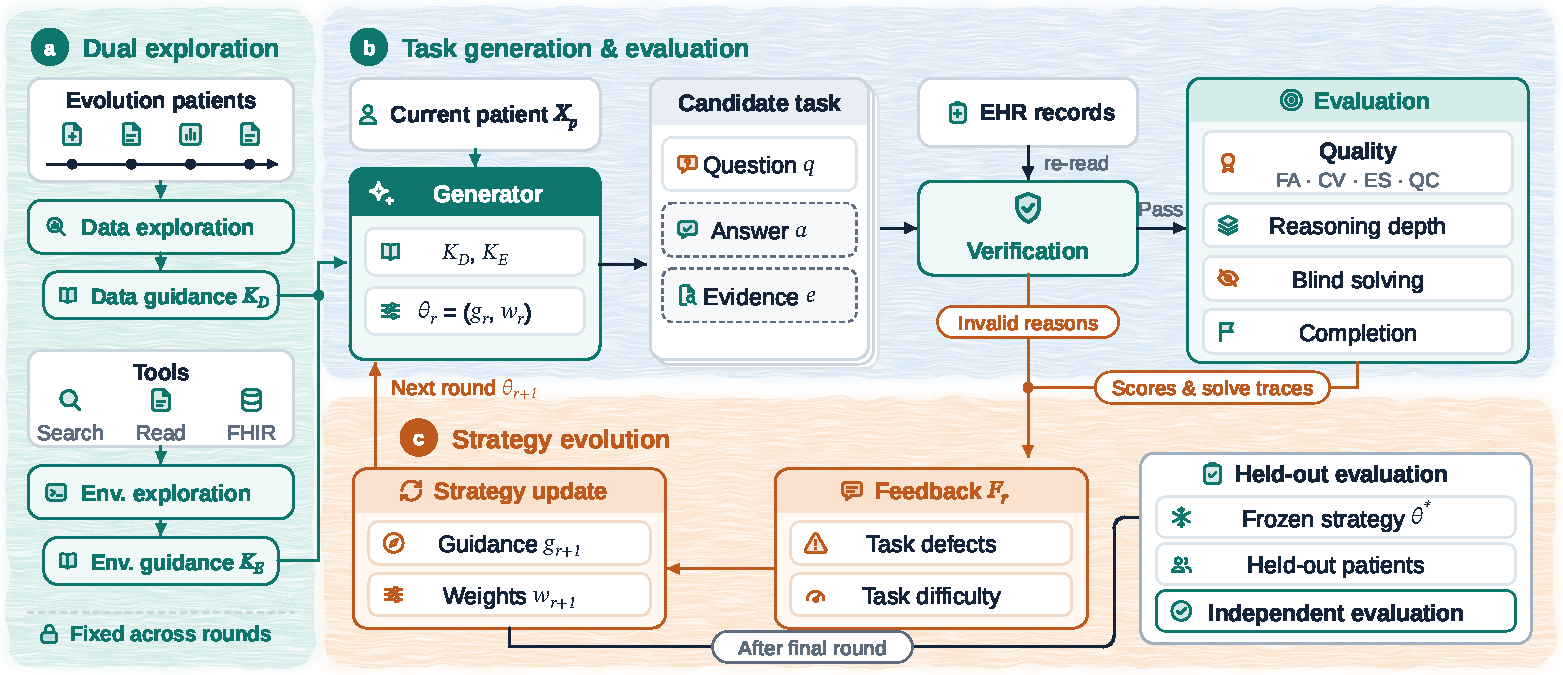
\includegraphics[width=\textwidth]{figures/medevolve-overview-v7.pdf}
\caption{Overview of MedEvolve. (a)~Dual exploration distills data guidance $K_D$ from the longitudinal records of evolution patients and environment guidance $K_E$ from read-only tool interaction, and both are reused unchanged in later rounds. (b)~The generator conditions on the current patient trajectory $X_p$, the two exploration guides, and the current strategy $\theta_r=(g_r,w_r)$ to produce candidate tasks, each comprising a question $q$, a reference answer $a$, and source evidence $e$; verification re-reads the original records, and tasks that pass proceed to quality (factual accuracy, FA; clinical validity, CV; evidence sufficiency, ES; question clarity, QC), reasoning depth, independent solving, and completion assessment, with reference answers and evidence claims withheld from the solving agent. (c)~Verification defects, evaluation scores, and solve traces jointly form feedback $F_r$, on which the strategy update revises the generation guidance $g_{r+1}$ and the direction weights $w_{r+1}$; after the scheduled rounds the strategy $\theta^*$ is frozen and evaluated on a held-out patient set.}
\label{fig:overview}
\end{figure*}

Longitudinal patient records document diagnoses, laboratory tests, medications, and other clinical events across multiple encounters, and they are the primary data source for building electronic health record (EHR) agent tasks; MedAgentBench~\citep{jiang2025medagentbench} and PhysicianBench~\citep{liu2026physicianbench} evaluate LLM agents in exactly such environments. Tasks of this kind usually require clinical experts to design and review them, which makes large-scale expansion difficult. On the automatic synthesis side, TaskCraft~\citep{shi2025taskcraft} generates tasks from web pages, PDFs, and images and increases task complexity through depth and width expansion, whereas CuES~\citep{mai2025cues} synthesizes tasks by interacting with and exploring the environment, with experiments spanning AppWorld, WebShop, and BFCL. Neither work is designed around the longitudinal structure of EHRs, nor around the constraint that a task's evidence must be retrievable through read-only tools.

Automatically constructing tasks on longitudinal records poses two specific difficulties. First, whether a task holds depends on both the case records and the environment tools. When the generator reads the current patient's trajectory, it sees only which records that patient carries; it cannot see which clinical relationships recur across the same data source, nor which resources typically hold the evidence for each type of question, and the full trajectory may itself exceed the model's input budget. A case with repeated test results, for example, can support trend-analysis questions, whereas a case dominated by diagnostic records suits clinical-interpretation questions better. At the same time, the evidence a question requires must be retrievable through the tools the environment exposes, which can only be established by actually calling those tools. Second, fixed generation guidance does not produce stable task quality and difficulty across cases, and its defects often surface only after evidence verification or after an agent actually attempts to solve the task.

We propose MedEvolve to address both points. Before generation, data exploration distills reusable clinical event patterns from longitudinal records, while environment exploration checks how evidence is obtained by calling read-only tools; together they constrain the generation of questions, reference answers, and source evidence. After generation, the system verifies evidence claims against the original records and has an independent agent solve the tasks, then aggregates verification defects, quality and reasoning scores, and solve traces into feedback that revises the natural-language generation guidance across patient batches and adjusts the sampling weights of different task directions. The whole process updates no model parameters.

Our contributions are: (1) combining data exploration with environment exploration so that task generation is constrained by both case content and tool capability; (2) using verification and solving feedback to update the generation strategy across patients without updating model parameters; and (3) providing an evaluation protocol covering valid yield, quality, reasoning requirements, and downstream experience learning, and testing these mechanisms in two EHR agent environments.

\section{Method}

\subsection{Problem Setting}

Given a medical environment $\mathcal{E}$ and a set of longitudinal patient trajectories $\mathcal{D}=\{X_p\}$, the goal is to construct a medical agent task for each trajectory $X_p$. Each task consists of an instruction $q$, a candidate reference answer $a$, and source evidence $e$. Generation is controlled by a strategy $\theta_r=(g_r,w_r)$, where $g_r$ is natural-language generation guidance, $w_r$ holds sampling weights over task types and difficulty directions, and $r$ is the evolution round. MedEvolve first obtains data guidance $K_D$ and environment guidance $K_E$ through exploration, then updates $\theta_r$ using evaluation feedback. Figure~\ref{fig:overview} shows the overall pipeline.



\subsection{Data and Environment Exploration}

A single patient's trajectory shows only which records that case contains, which makes it hard to tell what pattern those records follow across the whole data source, and reading a large number of patients again at every generation step is infeasible. We therefore run data exploration before generation and organize cross-patient observations into reusable guidance.

\textbf{Data exploration} targets longitudinal patient trajectories. The exploration agent reads the records of multiple patients, analyzes how the data are organized, how they change over time, how clinical events relate to one another, and how evidence is distributed, and distills the information patterns required by different task types into data guidance $K_D$. $K_D$ describes only reusable patterns and contains no patient-specific clinical facts.

\textbf{Environment exploration} targets the environment interface. The exploration agent actually calls read-only query tools and records access methods, return structures, and interaction constraints into environment guidance $K_E$, which serves to judge whether the evidence a question requires can be obtained through the tools.

Both explorations are completed during initialization and remain unchanged in all subsequent rounds.

\subsection{Task Generation and Evaluation}

For patient $X_p$, the generator conditions on $K_D$, $K_E$, and the current strategy $\theta_r$, and generates $(q,a,e)$ according to the specified task type and difficulty direction, where key facts carry references to the original records.

Candidate tasks then pass through verification, scoring, and independent solving in sequence. Verification re-reads the original records and checks that the evidence claims support the reference answer; tasks that pass verification are then assessed for task quality and reasoning depth and answered independently by a fixed agent in the environment. The solving agent has no access to reference answers or evidence claims.

\subsection{Feedback-Driven Strategy Updates}

After each round, the system aggregates that round's verification defects, quality and reasoning scores, and solve traces, and attributes them into feedback $F_r$. Attribution must separate defects of the task itself (such as factual errors, insufficient evidence, or ambiguous questions), the genuine reasoning difficulty the task poses, and model, tool, or environment failures, so that execution anomalies are not mistaken for task difficulty. The strategy is updated as
\begin{equation}
\theta_{r+1}=\mathcal{U}(\theta_r,F_r),
\end{equation}
where $\mathcal{U}$ is implemented by an LLM. The update acts on two parts: it writes generalizable construction experience into $g_{r+1}$, adjusting the selection of clinical information, the organization of evidence, and task design; and it adjusts $w_{r+1}$ according to the quality and difficulty performance of each direction, changing the direction distribution of subsequent tasks.

Different rounds use different patient batches to generate tasks. After the scheduled rounds the strategy is frozen and evaluated on a held-out patient set.

\section{Experiments}

\begin{table*}[!t]
\centering
\setlength{\tabcolsep}{7pt}
\renewcommand{\arraystretch}{1.15}
\begin{tabular*}{\textwidth}{@{\extracolsep{\fill}}lrrrr@{}}
\toprule
 & \multicolumn{2}{c}{PhysicianBench} & \multicolumn{2}{c}{MedAgentBench} \\
\cmidrule(lr){2-3}\cmidrule(lr){4-5}
Method & HO count (yield) & Mean level & HO count (yield) & Mean level \\
\midrule
\textbf{MedEvolve} & \textbf{23 (14.2\%)} & 2.27 & \textbf{77 (51.3\%)} & \textbf{2.73} \\
EnvExplore & 21 (13.0\%) & 2.25 & 64 (42.7\%) & 2.56 \\
TaskCraft & 0 (0.0\%) & 1.01 & 0 (0.0\%) & 1.00 \\
Workflow & 3 (1.9\%) & \textbf{2.30} & 2 (1.3\%) & 2.67 \\
SingleShot & 3 (1.9\%) & 1.20 & 11 (7.3\%) & 1.44 \\
SelfRefine & 4 (2.5\%) & 2.20 & 2 (1.3\%) & 2.00 \\
\bottomrule
\end{tabular*}
\caption{Valid higher-order task generation with GPT-5.4-nano. Higher-order (HO) tasks pass evidence verification and have an aggregate level of at least 3. Yield, shown in parentheses, uses the fixed number of requested tasks as its denominator (162 for PhysicianBench; 150 for MedAgentBench). Mean level covers all verified tasks with difficulty scores. Bold indicates the highest value in each column.}
\label{tab:exp1}
\end{table*}

\subsection{Experimental Setup}

\textbf{Environments and patients.} We evaluate on PhysicianBench and MedAgentBench. PhysicianBench contains 108 patients with clinical records. Of the 695 patients in MedAgentBench, 100 have clinical records, and we use these 100 patients. With seed~42, we partition PhysicianBench into 27 patients for evolution and 81 for held-out evaluation; the corresponding split for MedAgentBench is 25 and 75. The two sets are patient-disjoint. All methods share the evaluation patients and generate at most two read-only tasks per patient, giving 162 and 150 requested tasks, respectively. Appendix~\ref{app:splits} provides the full splits and information-access rules.

\textbf{Methods and generation model.} We compare six methods: MedEvolve, TaskCraft, Workflow, SingleShot, SelfRefine~\citep{madaan2023selfrefine}, and EnvExplore. Their procedures are described in Appendix~\ref{app:methods}. The generation model is GPT-5.4-nano. MedEvolve uses the full strategy after two update rounds, including generation guidance, task-direction descriptions, and weights. The two rounds use 13 and 14 evolution patients in PhysicianBench, and 12 and 13 in MedAgentBench. Methods differ in their call sequences and computational expenditure; the same task-count limit does not imply equal computational cost.

\textbf{Evaluation and metrics.} Generated tasks are first verified against the original records and then evaluated for reasoning difficulty. GPT-4o-mini and GPT-5.4-nano independently assign difficulty scores; we take the median and round down to obtain an aggregate level from 1 to 4. Scores reflect the minimum sufficient reasoning required to solve a task. Multiple pieces of evidence, a long temporal span, a lengthy answer, or missing information do not by themselves imply higher-order reasoning. We define a higher-order task as one that passes verification and has an aggregate level of at least 3. Experiment~1 uses three metrics:
\begin{itemize}
\item \textbf{Higher-order task count}: the number of verified tasks with an aggregate level of at least 3.
\item \textbf{Higher-order yield}: the higher-order task count divided by the fixed number of requested tasks, accounting for losses due to generation failures and invalid tasks.
\item \textbf{Mean level of valid tasks}: the mean level across all verified tasks with difficulty scores, rather than only higher-order tasks; this is an auxiliary metric.
\end{itemize}
Appendix~\ref{app:denominators} specifies the denominators, and Appendix~\ref{app:scoring} provides the scoring criteria.

\subsection{Experiment 1: Generating Valid Higher-Order Tasks}

This experiment evaluates whether a method produces more verified higher-order tasks under a shared patient set and per-patient task limit. Table~\ref{tab:exp1} reports results with GPT-5.4-nano as the generation model.



MedEvolve achieves the highest valid higher-order task yield among the six methods in both PhysicianBench and MedAgentBench, producing 23 and 77 verified higher-order tasks, with yields of 14.2\% and 51.3\%, respectively (Table~\ref{tab:exp1}). It produces more higher-order tasks in both environments than SingleShot (3 and 11) and SelfRefine (4 and 2). EnvExplore is the closest baseline, producing 21 and 64 tasks. MedEvolve produces 2 and 13 additional higher-order tasks, with yield differences of 1.2 and 8.6 percentage points, respectively.

Higher-order yield uses the fixed number of requested tasks as its denominator and accounts for both generation and verification failures. It therefore measures the ability of the full generation pipeline to deliver valid higher-order tasks. TaskCraft produces no higher-order tasks in this evaluation, with a mean level close to 1 among valid tasks. Workflow and SelfRefine generate relatively few tasks and also have low higher-order counts. MedEvolve has a lower verification pass rate than some baselines, but retains the largest number of higher-order tasks after verification and difficulty screening. Verification pass rate and valid higher-order yield thus capture different generation objectives; evaluating the final output requires considering its reasoning demands alongside validity.

Mean level provides an auxiliary perspective. MedEvolve achieves the highest mean of 2.73 on MedAgentBench. On PhysicianBench, its mean of 2.27 is close to Workflow's 2.30, which is based on 10 verified tasks. Taken together, higher-order counts, yields, and mean levels show that MedEvolve's main advantage is producing more tasks that combine higher reasoning demands with valid evidence under the same patient set and per-patient task limit.

\subsection{Experiment 2: Supplementing Official Training Tasks with Synthetic Tasks}

\begin{table}[!htbp]
\centering
\small
\setlength{\tabcolsep}{3pt}
\begin{tabular}{@{}lccc@{}}
\toprule
Framework & Official & Official + & $\Delta$ (pp) \\
 & 20 & Synthetic 40 & \\
\midrule
ACE & 4.0\% & 10.0\% & $+6.0$ \\
 & (2/50) & (5/50) & \\
Reflexion & 12.0\% & 14.0\% & $+2.0$ \\
 & (6/50) & (7/50) & \\
OpenClaw & 24.0\% & 20.0\% & $-4.0$ \\
 & (12/50) & (10/50) & \\
\bottomrule
\end{tabular}
\caption{Task success rates before and after adding synthetic tasks to official training tasks. Success requires the entire task to pass; all rates use the 50 planned test tasks as the denominator. Differences are in percentage points (pp).}
\label{tab:exp2}
\end{table}

This experiment evaluates whether adding MedEvolve-generated tasks to official training tasks improves agent performance on official test tasks. We compare ACE, Reflexion~\citep{shinn2023reflexion}, and OpenClaw in PhysicianBench. The execution model is Qwen3.8-27B with thinking disabled. Model parameters remain fixed, and each framework accumulates experience from training tasks through its own memory, reflection, or strategy mechanism.

We compare two training settings. \emph{Official 20} uses 20 official tasks. \emph{Official + Synthetic 40} adds 20 verified MedEvolve-generated tasks to the same 20 official tasks, with 10 synthetic tasks generated by GPT-4o-mini and 10 by GPT-5.4-nano. Both settings are evaluated on the same 50 official test tasks, with a model-call budget of 100 and seed~42. Reference answers are used only for scoring and are withheld from execution and learning. Experience is frozen after training and before testing. Appendix~\ref{app:harness} describes the framework mechanisms and evaluation protocol.



Adding MedEvolve-generated tasks increases the task success rates of ACE and Reflexion on the shared official test set (Table~\ref{tab:exp2}). ACE improves from 4.0\% (2/50) to 10.0\% (5/50), a gain of 6.0 percentage points; Reflexion improves from 12.0\% (6/50) to 14.0\% (7/50), a gain of 2.0 points. OpenClaw decreases from 24.0\% (12/50) to 20.0\% (10/50), a drop of 4.0 points. For scoring coverage, ACE has 48 scored tasks in the official-only setting and 50 in the mixed setting. Both settings of the other frameworks cover all 50 tasks. All reported success rates use the planned test-task count as the denominator.

These results suggest potential value for synthetic tasks in some experience-learning frameworks: with model parameters fixed and experience frozen during testing, ACE and Reflexion complete more official test tasks after training is supplemented with synthetic tasks. The decrease for OpenClaw shows that this improvement does not occur in every evaluated framework. The frameworks use different experience representations and update mechanisms, and the observed differences suggest that the benefits of synthetic tasks may depend on how experience is distilled and applied.

\raggedbottom

\section{Conclusion}

We present MedEvolve, which combines data and environment exploration to ground medical agent task generation in longitudinal patient records and tool-based evidence access. Verification and independent-solving feedback update generation guidance and task-direction weights across patients, without updating model parameters.

On PhysicianBench and MedAgentBench, MedEvolve achieves the highest valid higher-order task yield among the six compared methods, producing 23 and 77 verified higher-order tasks, respectively. Downstream experience-learning experiments further suggest potential value for synthetic tasks in some frameworks: adding synthetic tasks improves official-test success rates for ACE and Reflexion, but reduces the rate for OpenClaw, indicating differences in benefits across frameworks. These findings support dual exploration as an approach to constructing higher-order medical agent tasks and provide an empirical basis for studying how synthetic tasks interact with experience-learning mechanisms.

\section*{Limitations}

This study primarily evaluates the task-generation performance of the complete MedEvolve framework. Component ablations and round-by-round comparisons have not yet quantified the separate contributions of data exploration, environment exploration, feedback updates, and task-direction weights. The results characterize valid higher-order task yield under the full strategy; the individual effects of these mechanisms and their interactions require further investigation.

The downstream experience-learning experiment compares training on 20 official tasks with training on those tasks plus 20 synthetic tasks, changing both task count and composition. Controls using an equal number of official tasks or tasks produced by other generation methods would help distinguish the effects of training-set size from those of synthetic-task characteristics. The current downstream results come from a single seed and 50 test tasks in PhysicianBench; the stability of the gains and their performance in other environments require further evaluation.

MedEvolve derives generation guidance from patient records and tool interfaces within a particular environment. The current held-out patient evaluation examines strategy transfer within that environment. The applicability of existing guidance, and the adaptations it requires when healthcare institutions, record structures, or evidence-retrieval tools change, have not yet been systematically evaluated.

\clearpage
\appendix

\section{Exploration and Generation Interfaces}
\label{app:interfaces}

\subsection{Data Exploration}
\label{app:data-explore}
Exploration tools expose open patient IDs, budgeted trajectories, and optional compressed summaries. Inputs retain patient identifiers, source pointers, and coverage flags; the output is patient-agnostic natural-language guidance $K_D$. The guide summarizes data organization, temporal change, event relations, evidence citation patterns, and supportable questioning conditions, without retaining individual clinical values or source IDs.

Compressed summaries locate candidate patterns; original records support concrete claims. Missing records and budget truncation are stated separately. Time windows, record counts, and clinical relations in $K_D$ are inductive questioning constraints, not hard-coded medical rules applied uniformly across patients.

\subsection{Environment Exploration}
\label{app:env-explore}
Environment exploration queries native read-only tools in an isolated instance over open patients. Guidance $K_E$ records validated parameters, return shapes, pagination and truncation behavior, and typical retrieval procedures, and distinguishes call failures from unverified capabilities. Patient-specific observations stay out of the shared guide.

\subsection{Guidance Revision Example}
\label{app:guidance-example}
\begin{figure}[!t]
\centering
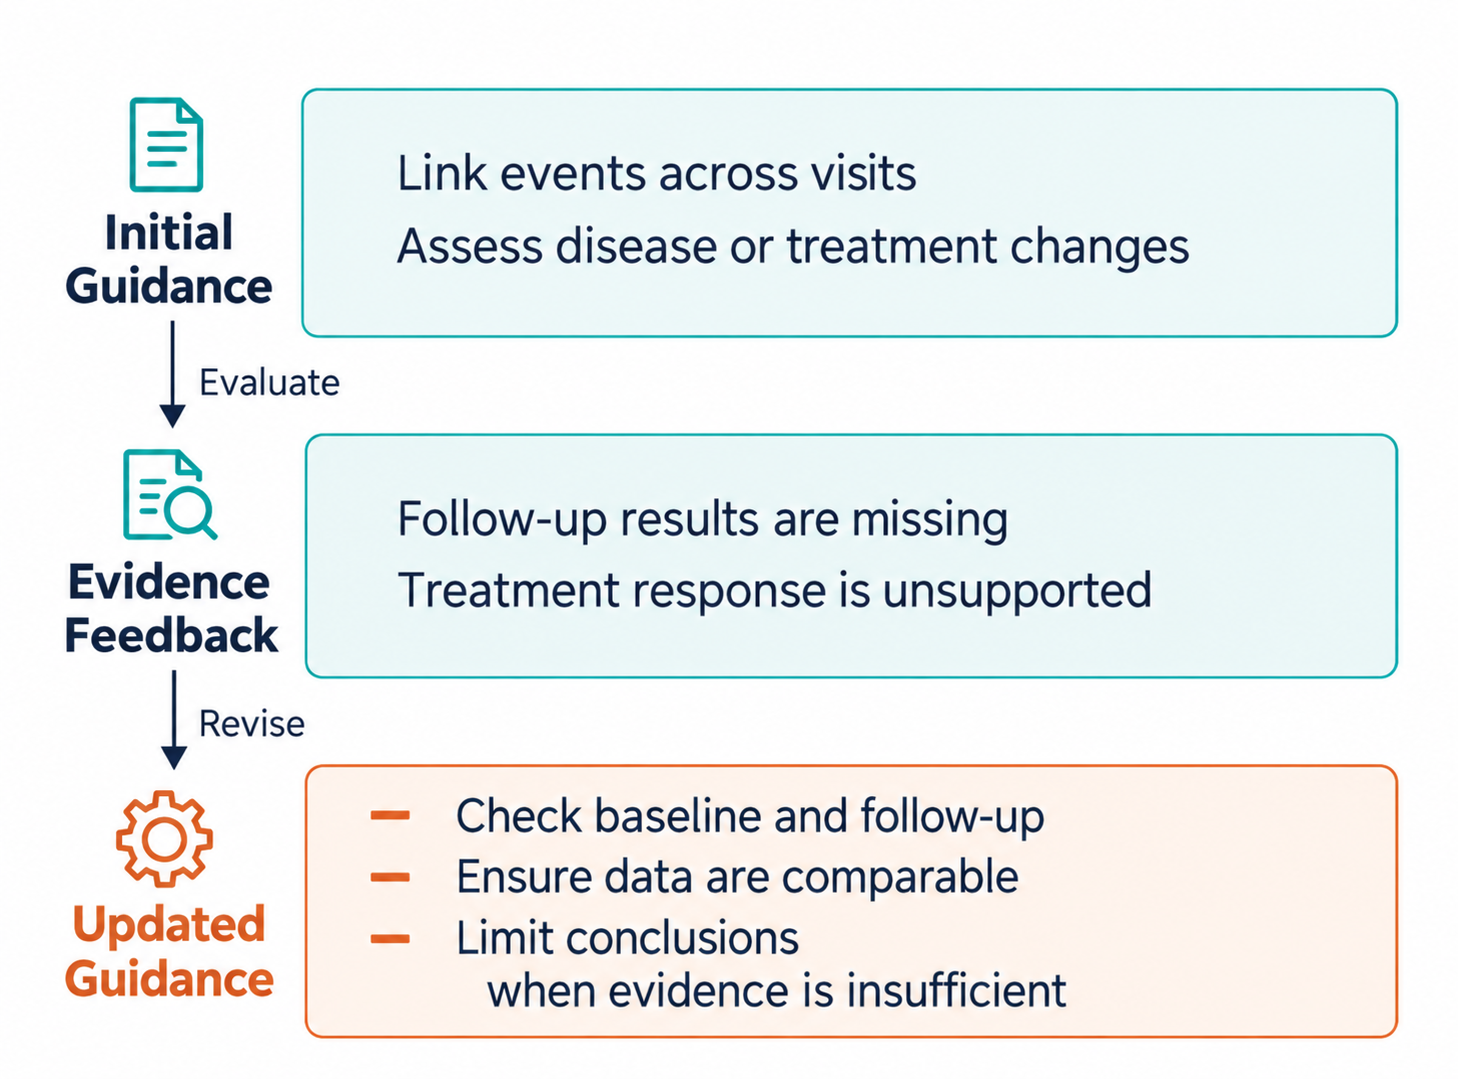
\includegraphics[width=\columnwidth]{figures/medevolve-strategy-example-en.png}
\caption{Example feedback-driven revision of generation guidance $g_r$. Verification feedback flags insufficient follow-up evidence; the revised guidance adds baseline/follow-up and comparability checks and restricts conclusions when evidence is weak. The example illustrates how $g_r$ can change, not that updates improve held-out metrics. Text is paraphrased from one evolution trace.}
\label{fig:app-guidance}
\end{figure}

\subsection{Task Generation and Strategies}
\label{app:gen-strategy}
A task records patient ID, clinical category, question, candidate reference answer, source identifiers with per-source factual claims, and execution requirements. The shared generation interface leaves the temporal-view field empty and requires read-only execution. One generation call receives the budgeted trajectory, $K_D$, $K_E$, current guidance $g_r$, and two sampled directions $Z_{p,r}$, and returns at most two candidates.

The strategy is $\theta_r=(g_r,w_r)$ with natural-language guidance and direction weights over five clinical categories and difficulty descriptions. Directions are sampled proportional to weights (at least one positive). $K_D$ and $K_E$ stay fixed during updates; only $g_r$ and $w_r$ change. Evolution rounds sample from the current weights; held-out evaluation uses the frozen updated guidance, task-direction descriptions, and weights.

\section{Environments, Patients, and Information Access}
\label{app:splits}

\begin{table}[!t]
\centering
\small
\setlength{\tabcolsep}{4pt}
\caption{Generation-side patient splits (seed~42).}
\label{tab:app-splits}
\begin{tabular}{@{}lcccc@{}}
\toprule
Env & Pool & Evo. & Held-out & Rounds \\
\midrule
PhysicianBench & 108 & 27 & 81 & 13/14 \\
MedAgentBench & 100 & 25 & 75 & 12/13 \\
\bottomrule
\end{tabular}
\end{table}

Table~\ref{tab:app-splits} freezes evolution and held-out lists under seed~42 with prior exploration-exposure constraints; patients do not cross sets. Trajectories are ordered by record time and budgeted for model input; verification rereads original sources rather than input summaries. Initial exploration and generation expose query tools only. The public interface does not enable temporal-view isolation, so time language in a question does not hide later records server-side. The training and test split for Experiment~2 is separate from the generation-side patient split. Training uses 20 official tasks and, in the mixed setting, 20 verified synthetic tasks; both settings share 50 official test tasks. The frozen manifest records selected tasks, patients, splits, file hashes, and generation sources.

\section{Generation Methods and Budgets}
\label{app:methods}

TaskCraft maps patient records and read-only FHIR tools onto atomic extraction, verification, and depth/width expansion; both branches start from atomic tasks, share a generation budget, and record acceptance separately from final filtering. Workflow runs localize--generate--filter with filtering only. SingleShot emits at most two tasks in one pass. SelfRefine drafts, self-critiques, and revises within a patient batch (up to three critiques and two revisions; early stop on pass). EnvExplore obtains environment guidance once, then generates under a fixed initial strategy. MedEvolve uses dual exploration and the full strategy after two rounds of cross-patient feedback-driven updates. All methods share the output schema and external evaluation; internal calls and filters are logged separately.

Matching task counts are not treated as identical token budgets. Exploration and updates count toward MedEvolve cost; shared evaluation is reported separately; reused historical calls are deduplicated from original logs.

\section{Scoring, Aggregation, and Statistics}
\label{app:scoring}

\subsection{Quality and Reasoning Depth}
\label{app:quality}
Quality uses four 1--5 dimensions scored independently: factual accuracy (FA), clinical validity (CV), evidence sufficiency (ES), and question clarity (QC). Rough anchors: 5~=~fully accurate/supported/clear; 3~=~mostly correct with material gaps; 1~=~severe error, unsupported inference, or unusable question. Reasoning depth is labeled from task demand and evidence structure: (1)~factual retrieval, (2)~single-step judgment, (3)~cross-record integration, (4)~clinical decision-making; levels 3--4 count as higher-order (HO). Category and depth are recorded separately; treatment-planning items are not auto-labeled as level~4.

For task $i$ and dimension $d$, two judges yield $s_{i,d}^{(1)},s_{i,d}^{(2)}$; we take
\[
s_{i,d}=\left\lfloor\operatorname{median}\bigl(s_{i,d}^{(1)},s_{i,d}^{(2)}\bigr)\right\rfloor.
\]
Depth uses the same aggregation. The protocol requires two valid judge outputs; a single success does not impute a missing score.

\subsection{Evidence Structure and Rate Denominators}
\label{app:denominators}
Deduplicated cited sources $S_i$ give evidence count $|S_i|$; resource-type count uses recognizable type prefixes. Parseable timestamps $T_i$ define span $\Delta_i=(\max T_i-\min T_i)$ in days (missing if none; zero if one). Span summaries use non-missing values only.

Higher-order task count includes only verified tasks with an aggregate difficulty level of at least 3. Higher-order yield divides this count by the fixed requested-task count. Mean level divides the sum of aggregate levels by the number of verified tasks with difficulty scores. Verification pass rate divides the verified-task count by the actual generated-task count. Experiment~2 divides the number of fully successful test tasks by all 50 planned test tasks.

Generation failures and invalid tasks remain in yield accounting and are not removed from the denominator. Scoring failures in Experiment~2 are reported as missing coverage, rather than relabeled as success or failure. Zero denominators are reported as missing.

\subsection{Uncertainty}
\label{app:uncertainty}
The higher-order task comparisons in Experiment~1 do not include interval estimates. Experiment~2 uses one seed and 50 planned test tasks.

\section{Experience Learning and Official Evaluation}
\label{app:harness}

\begin{table*}[t]
\centering
\small
\setlength{\tabcolsep}{4pt}
\renewcommand{\arraystretch}{1.15}
\begin{tabularx}{\textwidth}{@{}lXXX@{}}
\toprule
Framework & Persisted experience & Training updates & Test state \\
\midrule
OpenClaw & Skills and an isolated state directory & Native Skill Workshop; whether it is triggered is recorded & Frozen skills; learning and background maintenance disabled \\
ACE & Playbook & Reflector and Curator updates & Generator only \\
Reflexion & Reflections and transferable experience & Failure reflection and a limited number of retries & Actor only, reading stored experience \\
\bottomrule
\end{tabularx}
\caption{Experience representations and update mechanisms of the three frameworks.}
\label{tab:app-harness}
\end{table*}

The two training settings maintain separate configurations and experience stores and start from the same initial state. Reflexion's cross-task experience distillation is adapted to the medical setting: it stores applicability conditions, operational steps, and lessons from errors, without patient identifiers, individual clinical values, or per-task answers. Each new task retrieves at most three relevant experience entries under frozen rules. Test-time scoring does not trigger reflection or retries.

The execution model is Qwen3.8-27B with thinking disabled, a model-call budget of 100, and seed~42. Both training settings share the same 20 official tasks. The mixed setting adds 20 verified MedEvolve-generated tasks, with 10 generated by GPT-4o-mini and 10 by GPT-5.4-nano.

PhysicianBench uses official tasks and checkpoint-based scoring, with actual file deliverables, execution traces, and the task's FHIR instance. Missing official assets or scoring errors are retained as unavailable results; shared LLM judgments do not replace native scores. Reference answers are used only for scoring and are withheld from execution and learning.

Test scoring is isolated from task solving, and the medical instance used for execution is retained until scoring finishes. Each task uses a copy of the frozen experience. Reference answers, scoring results, and full conversations are not written back to the final experience store. Experience hashes are checked before and after testing, and both the planned task count and scoring coverage are reported.

\section{Generation and Verification Counts}
\label{app:extra-results}

\begin{table*}[t]
\centering
\small
\setlength{\tabcolsep}{5pt}
\renewcommand{\arraystretch}{1.1}
\begin{tabular*}{\textwidth}{@{\extracolsep{\fill}}lrrrr@{}}
\toprule
 & \multicolumn{2}{c}{PhysicianBench} & \multicolumn{2}{c}{MedAgentBench} \\
\cmidrule(lr){2-3}\cmidrule(lr){4-5}
Method & Generated / verified & Pass rate & Generated / verified & Pass rate \\
\midrule
MedEvolve & 157 / 70 & 44.6\% & 146 / 104 & 71.2\% \\
TaskCraft & 128 / 125 & 97.7\% & 111 / 108 & 97.3\% \\
Workflow & 32 / 10 & 31.3\% & 11 / 3 & 27.3\% \\
SingleShot & 162 / 122 & 75.3\% & 150 / 127 & 84.7\% \\
SelfRefine & 12 / 10 & 83.3\% & 7 / 6 & 85.7\% \\
EnvExplore & 149 / 107$^\dagger$ & 71.8\%$^\dagger$ & 141 / 108 & 76.6\% \\
\bottomrule
\end{tabular*}
\caption{Generation and verification counts with GPT-5.4-nano from frozen earlier batches. Entries give actual generated and verified task counts; pass rate divides verified by generated tasks.}
\label{tab:counts}
\end{table*}

$^\dagger$ EnvExplore's PhysicianBench counts come from a frozen earlier batch, rather than the latest run that produced the 21 higher-order tasks in Table~\ref{tab:exp1}. These counts cannot serve as the denominator for those 21 tasks.

\section{Illustrative Cases}
\label{app:cases}

Author-verified illustrative cases are pending and are not included in this draft.\pending


\section*{Writing Assistance}
Manuscript organization and evidence-status checks were assisted by the scientific-writing skill from Scientific Agent Skills~\citep{kassis2026skills}. The authors remain responsible for verifying the literature and scientific claims.

\bibliography{references}
\end{document}
